\section{Scenario 2 - Curvature of the Earth}\label{sec:scenario2}
The purpose of this scenario is to simulate and show how the curvature of the Earth comes into play, as seen on the map in Figure \ref{fig:s2_map}. In this case, the UA starts near the GS and moves away from it in a somewhat straight line. To be mentioned that a PD controller is used in simulation of the UAS.

\begin{figure}[H]
	\hfill
	\subfigure[UAS Map Positioning]{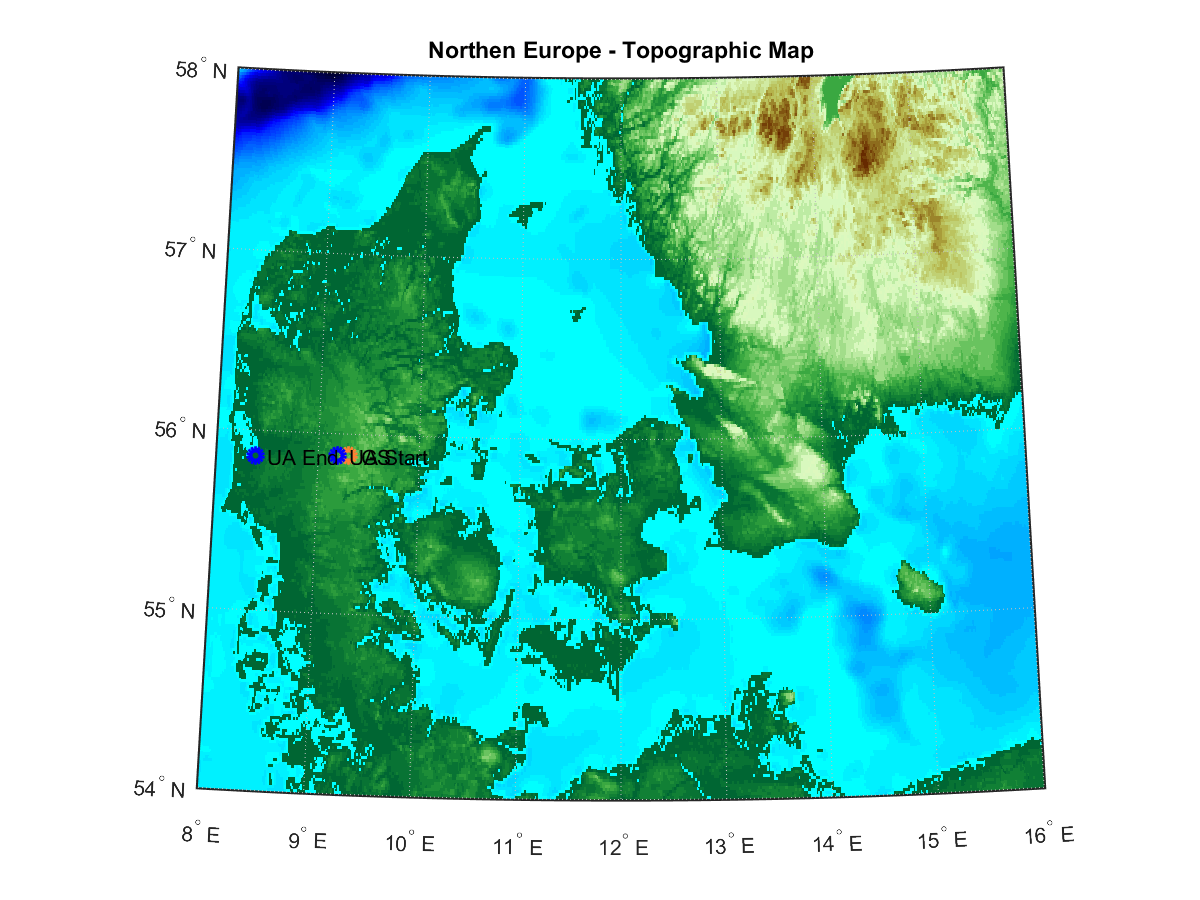
\includegraphics[scale=0.34]{figures/s2_map.png}}
	\hfill
	\subfigure[LOS and Distance]{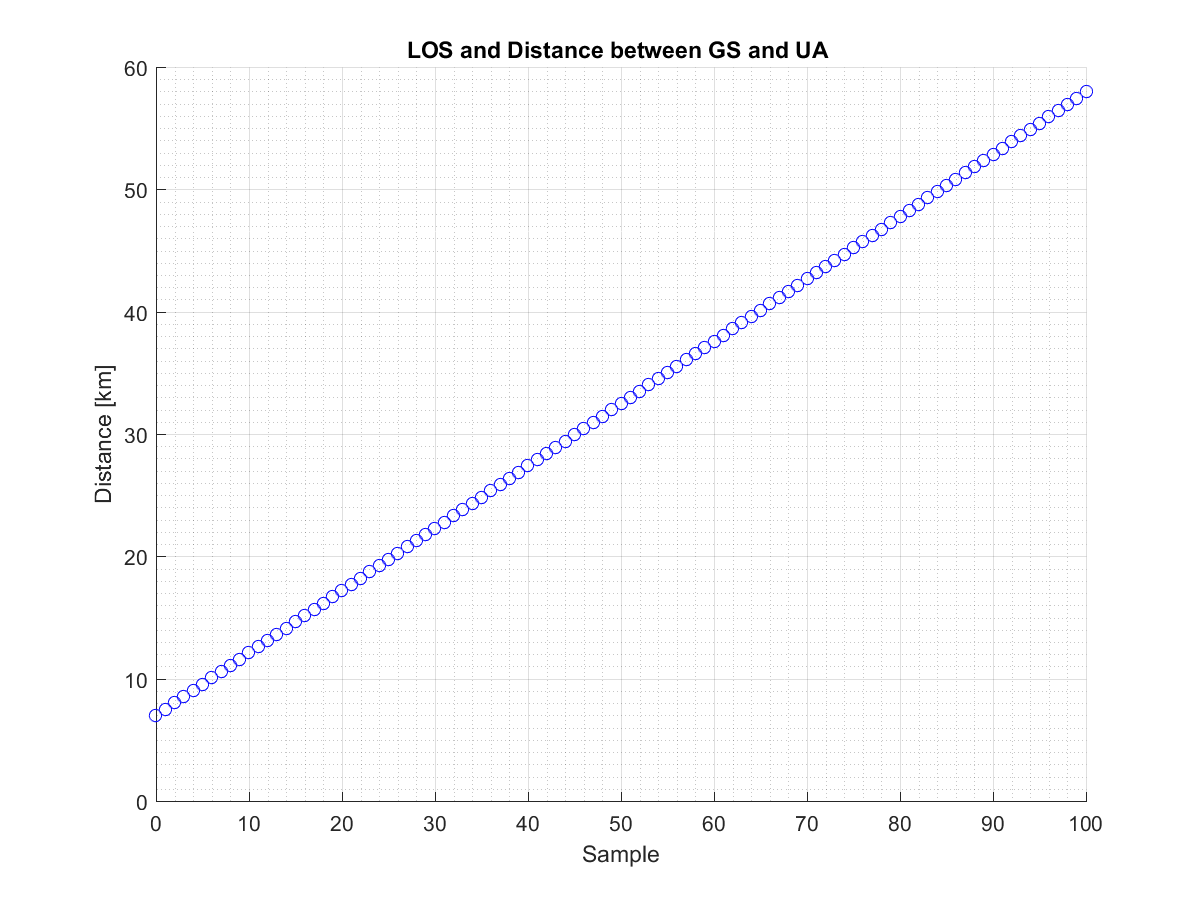
\includegraphics[scale=0.34]{figures/s2_los.png}}
	\hfill
	\caption{Mountain Scenario}
	\label{fig:s2_map}
\end{figure}


\subsection{Ground Station}
In Figure \ref{fig:s2_gs} the angle tracking of the GS antenna can be seen.

\begin{figure}[H]
	\centering
	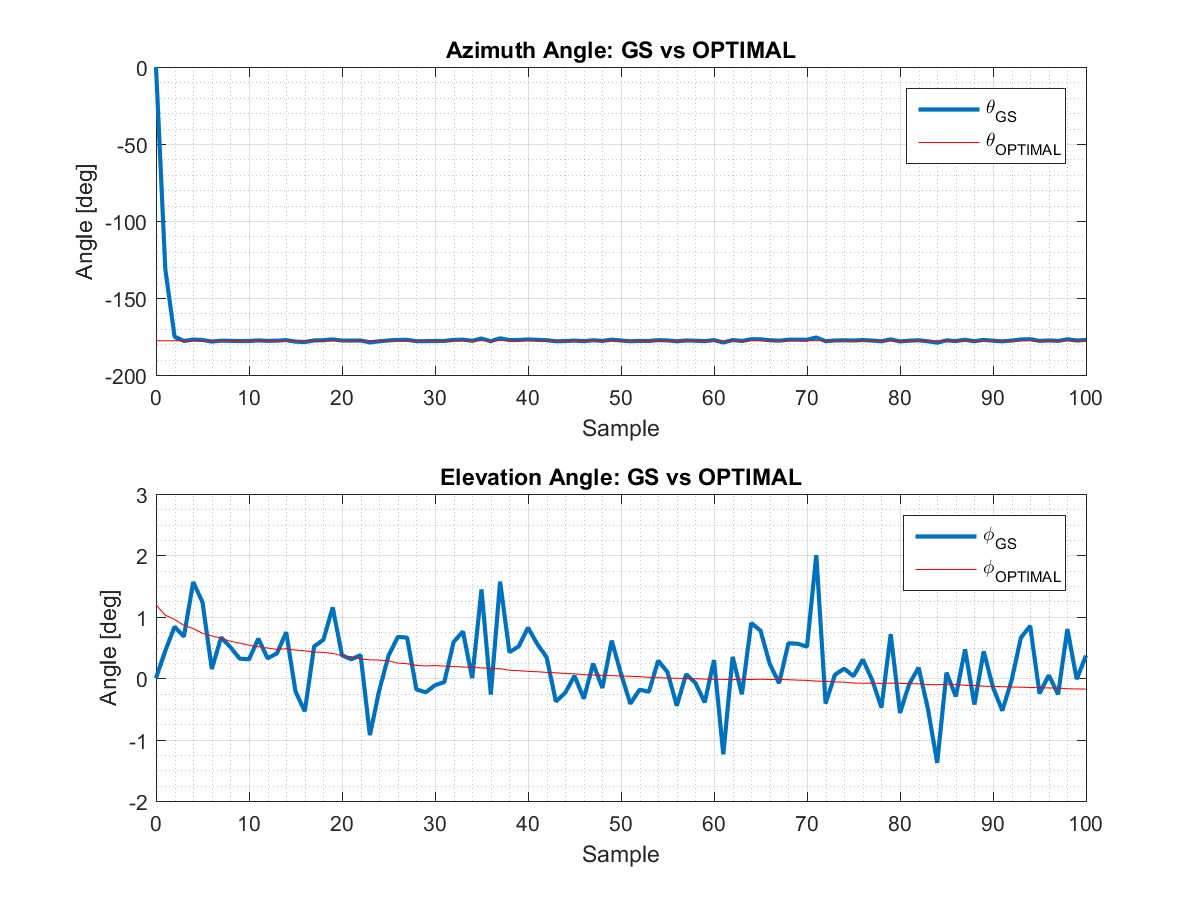
\includegraphics[scale=0.75]{figures/s2_gs.png}
	\caption{Azimuth and elevation angles of GS following the optimal angle}
	\label{fig:s2_gs}
\end{figure}

\subsection{Unmanned Aircraft}
In Figure \ref{fig:s2_ua} the angle tracking of the UA antenna can be seen.

\begin{figure}[H]
	\centering
	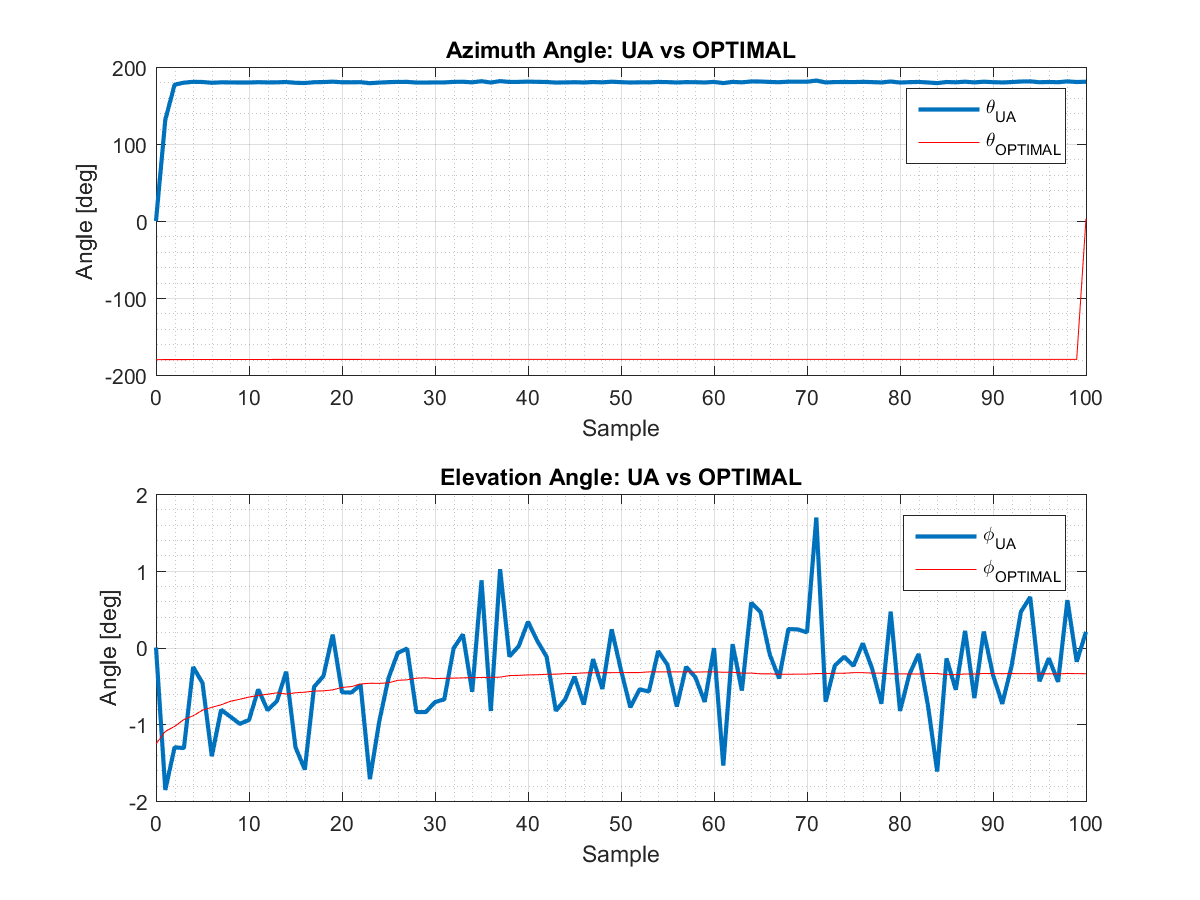
\includegraphics[scale=0.75]{figures/s2_ua.png}
	\caption{Azimuth and elevation angles of UA following the optimal angle}
	\label{fig:s2_ua}
\end{figure}


\subsection{Power}
In Figure \ref{fig:s2_power} the power at the receiver antenna of the GS antenna can be seen.

\begin{figure}[H]
	\centering
	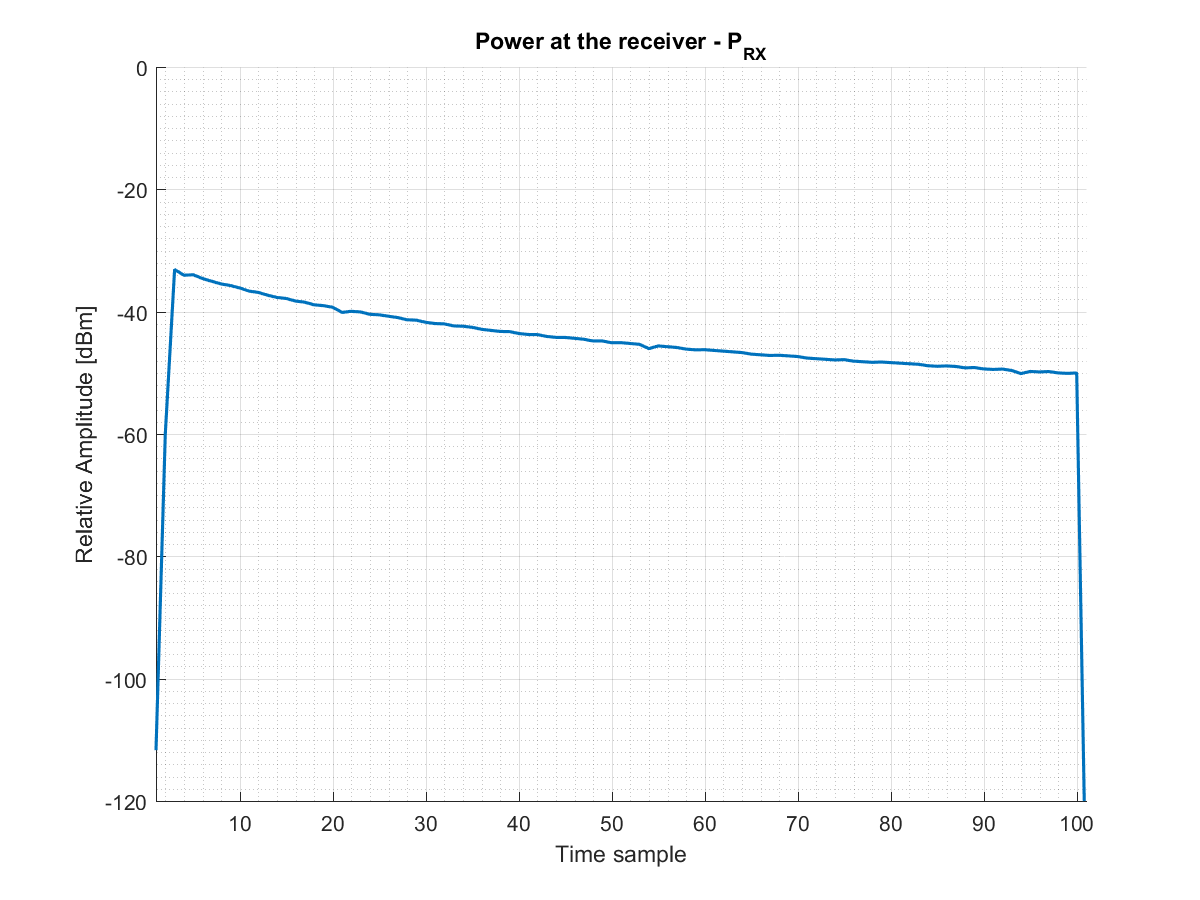
\includegraphics[scale=0.75]{figures/s2_power.png}
	\caption{Power at the receiver's antenna (GS)}
	\label{fig:s2_power}
\end{figure}

